\documentclass{report}

\title{\Large{\textbf{TMA template file}}}
\author{Richard Whittle {\textbf{U5512912}}}
\date{\today}

%\usepackage[margin=0.5in]{geometry}
\usepackage{pgfplots}
\usepackage{mathtools}
\usepackage{cancel}
\usepackage{pgfplots}
\usepackage{amsmath}
\newtheorem{theorem}{THEOREM}
\newtheorem{proof}{PROOF}
\usepackage{tikz}
\usetikzlibrary{arrows}
\usepackage{amssymb}
\usetikzlibrary{patterns}
\usepackage{bigints}
\usepackage{color}
\usepackage{tcolorbox}
\usepackage{booktabs,array}
\usepgfplotslibrary{fillbetween}

\usepackage{amsmath}
\usepackage{index}
\usepackage{fancyhdr}
%\usepackage{tikzpicture}
\usepackage{pgfplots}
%\usepackage{pifont}
%usepackage{xltxtra,xunicode}
\usepackage{soul,xcolor}
\makeindex

\pgfplotsset{compat=1.16}

\begin{document}

\begin{titlepage}
\maketitle
\end{titlepage}

\tableofcontents
\pagebreak

\pagenumbering{arabic}

\pagestyle{fancy}
\fancyhf{}
\rhead{Overleaf}
\lhead{MU123 19B}
\rhead{forename surname OU ID}
\rfoot{Page \thepage}

%start working after this

\subsection*{Source code here}

\subsection*{Strikethrough text}
\setstcolor{red}

\st{Some overstruck text}

\[ \frac{\cancel{3}.4^{n+1}}{\cancel{3}}\\ \]

\section{Drawing things}

\subsubsection{Draw a plain line}
 See fig:\ref{Example line drawing}
\begin{figure}[ht]
\begin{tikzpicture}
% Draw a line
\draw (0,0) -- (4,0);
\end{tikzpicture}
\caption{Example line drawing}
\label{Example line drawing}
\end{figure}



To draw a rectangle state the size x,y as shown in fig:\ref{Example rectangle drawing}

\begin{figure}[ht]
\begin{tikzpicture}
%\subsubsection{Draw a rectangle}
\draw (0,0) -- (6,0) -- (6,4) -- (0,4) -- cycle;
\end{tikzpicture}
\caption{Example rectangle drawing}
\label{Example rectangle drawing}
\end{figure}

To draw a parabola, state the co-ordinates as found in fig:\ref{Example parabola drawing}

\begin{figure}[ht]
\begin{tikzpicture}
% \draw (0,0) rectangle (6,4);
\draw (0,0) parabola (6,4);
\end{tikzpicture}
\caption{Example parabola drawing}
\label{Example parabola drawing}
\end{figure}

An example of an inequality may be found in fig:\ref{example inequality}

\begin{figure}[ht]
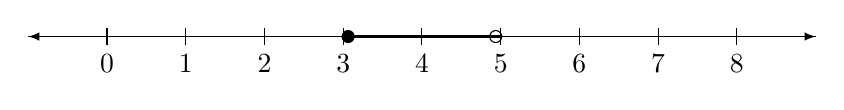
\begin{tikzpicture}
\draw[latex-] (-1,0) -- (9,0) ;
\draw[-latex] (-1,0) -- (9,0) ;
\foreach \x in  {0,1,2,3,4,5,6,7,8} \draw[shift={(\x,0)},color=black] (0pt,3pt) -- (0pt,-3pt);
\foreach \x in {0,1,2,3,4,5,6,7,8} \draw[shift={(\x,0)},color=black] (0pt,0pt) -- (0pt,-3pt) node[below] {$\x$};
\draw[*-o] (2.98,0) -- (5.02,0);
% * means includes (full circle), and o means excludes (empty circle)
\draw[very thick    ] (2.98,0) -- (5.02,0);
\end{tikzpicture}	
\caption{example inequality}
\label{example inequality}
\end{figure}


\begin{comment}
\subsubsection*{Source code here}
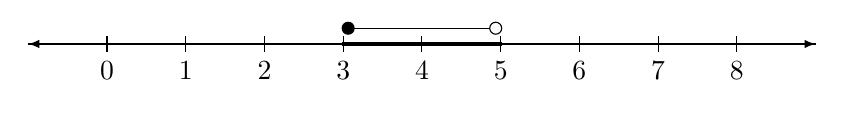
\begin{tikzpicture}
\draw[latex-] (-1,0) -- (9,0) ;
\draw[-latex] (-1,0) -- (9,0) ;
\foreach \x in  {0,1,2,3,4,5,6,7,8} \draw[shift={(\x,0)},color=black] (0pt,3pt) -- (0pt,-3pt);
\foreach \x in {0,1,2,3,4,5,6,7,8} \draw[shift={(\x,0)},color=black] (0pt,0pt) -- (0pt,-3pt) node[below] {$\x$};
\draw[*-o] (2.98,0.2) -- (5.02,0.2);
% * means includes (full circle), and o means excludes (empty circle)
\draw[very thick    ] (2.98,0) -- (5.02,0);
\end{tikzpicture}	
	
\end{comment}

An example of simple factor tree can be seen on the pages below in fig:\ref{Factor tree simple}
\begin{figure}[!hb]
    \centering
    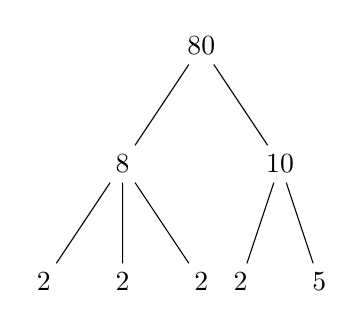
\begin{tikzpicture}[
        level 1/.style={sibling distance=20mm},
        level 2/.style={sibling distance=10mm},
    ]
    \node{80}
        child{node {8}
            child{node {2}}
            child{node {2}}
            child{node {2}}
        }
        child{node {10}
            child{node {2}}
            child{node {5}}
        };
    \end{tikzpicture}
    \caption{Simple tree}
    \label{Factor tree simple}
\end{figure}

An example of an elaborated factor tree can be seen below in fig:\ref{Factor tree elaborate} 

\begin{figure}[!ht]
    \centering
    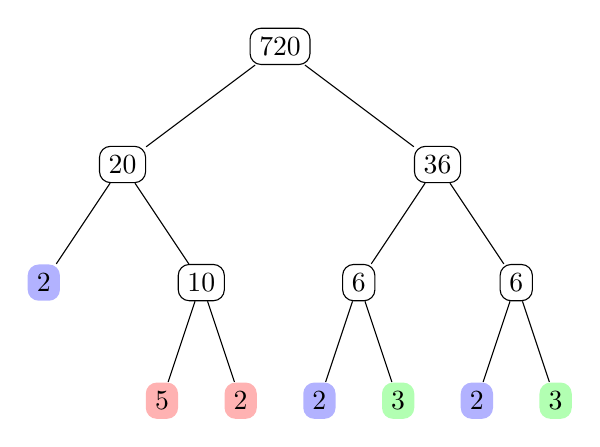
\begin{tikzpicture}[
        level 1/.style={sibling distance=40mm},
        level 2/.style={sibling distance=20mm},
        level 3/.style={sibling distance=10mm}
        ]
    \node[rounded corners, draw]{720}
        child{node [rounded corners, draw] {20}
            child{node [fill=blue!30,rounded corners] {2}}
            child{node [rounded corners, draw] {10}
                child{node [fill=red!30,rounded corners] {5}}
                child{node [fill=red!30,rounded corners] {2}}
            }
        }
        child{node [rounded corners, draw] {36}
            child{node [rounded corners, draw] {6}
                child{node [fill=blue!30,rounded corners] {2}}
                child{node [fill=green!30,rounded corners] {3}}
            }
            child{node [rounded corners, draw] {6}
                child{node [fill=blue!30,rounded corners] {2}}
                child{node [fill=green!30,rounded corners] {3}}
            }
        };
    \end{tikzpicture}
    \caption{Elaborated tree}
\label{Factor tree elaborate}
\end{figure}

\clearpage

\section{Unit x}

\subsection{Stratagy - details}

\subsection{Activity - details}

\subsubsection{(a) - question details}

\begin{itemize}
\item[i] specifics about the question
\item[ii] specifics about the question
\item[iii] specifics about the question
\end{itemize}

\end{document}